% Chapter 3
\chapter{Partitioning the Network}
\label{chapter3}
%--------------------------------------------------------------------------
\section {Introduction}

FPGAs have been extensively used for full system prototyping and verification of large ASIC designs. Lowering costs, as a consequence of advanced manufacturing processes and increasing competition, coupled with rising operating speeds, have rendered FPGA prototyping a considerable advantage over other known alternatives. These include RTL simulation and virtual prototyping, which are known to be slow and expensive in comparison. FPGAs make good use of available fine-grained parallelism and find applications in High Performance Computing (HPC) and hardware acceleration. A number of hardware/software co-simulation tools, such as ProtoFlex, have been developed which rely on FPGA for fast hardware emulation of complex designs and also provide testing and debugging support. Modern day customized chips, on the other hand, have also seen a remarkable rise in design complexity with advanced ASICs consisting of over a billion gates. Although FPGAs have also witnessed a rapid increase in integration costs, resource constraints in terms of limited gate capacity, DSP units, I/O pins, memory arrays and clock speeds render FPGAs almost impractical for prototyping of very large designs using a single chip. To mitigate this issue, the large ASIC designs are often partitioned across multiple FPGAs such that the major functional blocks reside over different FPGAs, which are further provisioned with an appropriate communication interface. Multi-FPGA partitioning is still considered to be one of the toughest challenges in FPGA prototyping. It is cumbersome and error-prone as it requires considerable manual intervention and knowledge of partitioned modules. To this end, we believe that a standardized and simplified communication interface based on Network-on-chip (NoC), with automated partitioning across multiple FPGAs, could greatly allay the designers from the tedious partitioning process. The partitioned NoC should also be flexible in terms of topology and routing configurations. Since several modern day ASICs and MPSoCs also employ NoCs for communication between modules, our partitioned NoC would also be effective for prototyping and debugging of these designs on multiple FPGAs, which are otherwise limited by the resource constraints of a single FPGA. This approach is also handy for designing multiple FPGA-based hardware accelerators, using the underlying NoC as the communication interface.\\
\section {NoC partitioning}

Partitioning of network is a very useful technique which provides opportunities to test large ASIC and SoC which are not able to fit in a single chip/FPGA. The challenges of partitioning an application for multi-chip system requires large number of IO. To overcome these challenges we partition CONNECT generated NoC into desired number of node in each partition and instantiate high speed serial or partial serial links in the partitioned instances. Figure VIII shows 2 $\times$ 2 mesh partitioned into 2 instances and also the high speed serial links between them\footnote{The core idea of this NoC partitioning is from Yatish's DDP where he used the same partitioning methods as explained in the Chapters below using UART serial link for the communication between two partitioned networks.}.\\
\section {Automated partitioning script}

To partition the NoC we initially used manual partitioning method. While performing the manual partitioning we noted all the interconnections and routing table dependencies of each port of each router. This help us developing the automated method of partitioning the NoC by giving specific details about the cuts needed in the network. This automation is done by a python script \cite{yatish_ddp} which takes in total number of router, partition number, number of routers in each partition and the original un-partitioned NoC as input. This script learns first about the original network about the port connection between each router to other router. \\

\section {Router Details}

Each router in this generated network consist of 5 ports each port has the following interfacing pins:
\begin{table} [H]
\caption{Router Pins}
\begin{center}
 \begin{tabular}{||c | c||} 
 \hline
    \textbf{PIN} & \textbf{DESCRIPTION} \\ \hline
	in\_ports\_$<$PORT$>$\_putRoutedFlit\_flit\_in & Input data to router\\
	EN\_in\_ports\_$<$PORT$>$\_putRoutedFlit & Enable to receive from the input port\\
	EN\_in\_ports\_$<$PORT$>$\_getNonFullVCs & Enable for virtual channel for this port\\
	in\_ports\_$<$PORT$>$\_getNonFullVCs & Input information of non-full VC \\
	EN\_out\_ports\_$<$PORT$>$\_getFlit & Output port enable\\
	out\_ports\_$<$PORT$>$\_getFlit & Output data from router\\
	out\_ports\_$<$PORT$>$\_putNonFullVCs\_nonFullVCs & VC information for output port\\
	EN\_out\_ports\_$<$PORT$>$\_putNonFullVCs & Enable for out port VC\\
 \hline
\end{tabular}
\end{center}
\label{RouterPins}
\end{table}

Input data from the router is sent to Quasi-SERDES physical link module, the enable signals to the router indicating the status of the Quasi-SERDES help to manage the data flow and handshake between the interfaces. This Quasi-SERDES is a transceiver link, cross connected to another similar SERDES module. The Figure \ref{PartionedNoC} show the network after partitioning with Quasi-SERDES link module instantiated. The script exposes the Quasi-SERDES link connections in the partitioned network. This exposed Quasi-SERDES links have to connect to exposed pads of other half of the partitioned network. Appendix A-4 gives details of the python scripts.


\begin{centering}
\begin{figure}[H]
  \centering
   \includegraphics[scale=1]{./figs/PartitionedNoC2x2}
  \caption{\textbf{Partitioned Network with inter chip communication interface}}
  \label{PartionedNoC}
\end{figure}
\end{centering}

\section {Example of data route between router ports}

Let us now exercise an example in this set-up. Below is a data flit structure injected in a router port.\\
\begin{centering}\textit{$<$1/*Valid*/, 0/*Tail*/, 11/*Destination*/, 0/*VC*/, 1010101111/*Data*/$>$}\end{centering}

The flit traverses in exactly the same manner till the router 2 port 3 as explained in Section 2.4. For Aurora IP Core as physical link interface, when the flit arrives at port 3 of Aurora module, it undergoes encoding based on Aurora 8B10B protocol, serialization conversion and then transmitted. This serial data is then transmitted from specialized high speed multi-gigabyte transceiver (MGT) IOs which is received on the similar MGT on the counter part in the second partition. This received serial data is the converted into parallel data and decoded to form the original flit. And finally when it reaches the destination router the flit is pushed out from port 0 of router 3.\\ 

When the Quasi-SERDES modules are interfaced in between 2 routers then the data flit gets buffered and then transmitter 8 bits in one clock cycle with MSB first and similarly received by receiver port of Quasi-SERDES link and stored in output buffer and ejected out from the out port to the router. This take 10 clock cycles for 24 bit flit. \\


\begin{centering}
\begin{figure}[H]
  \centering
   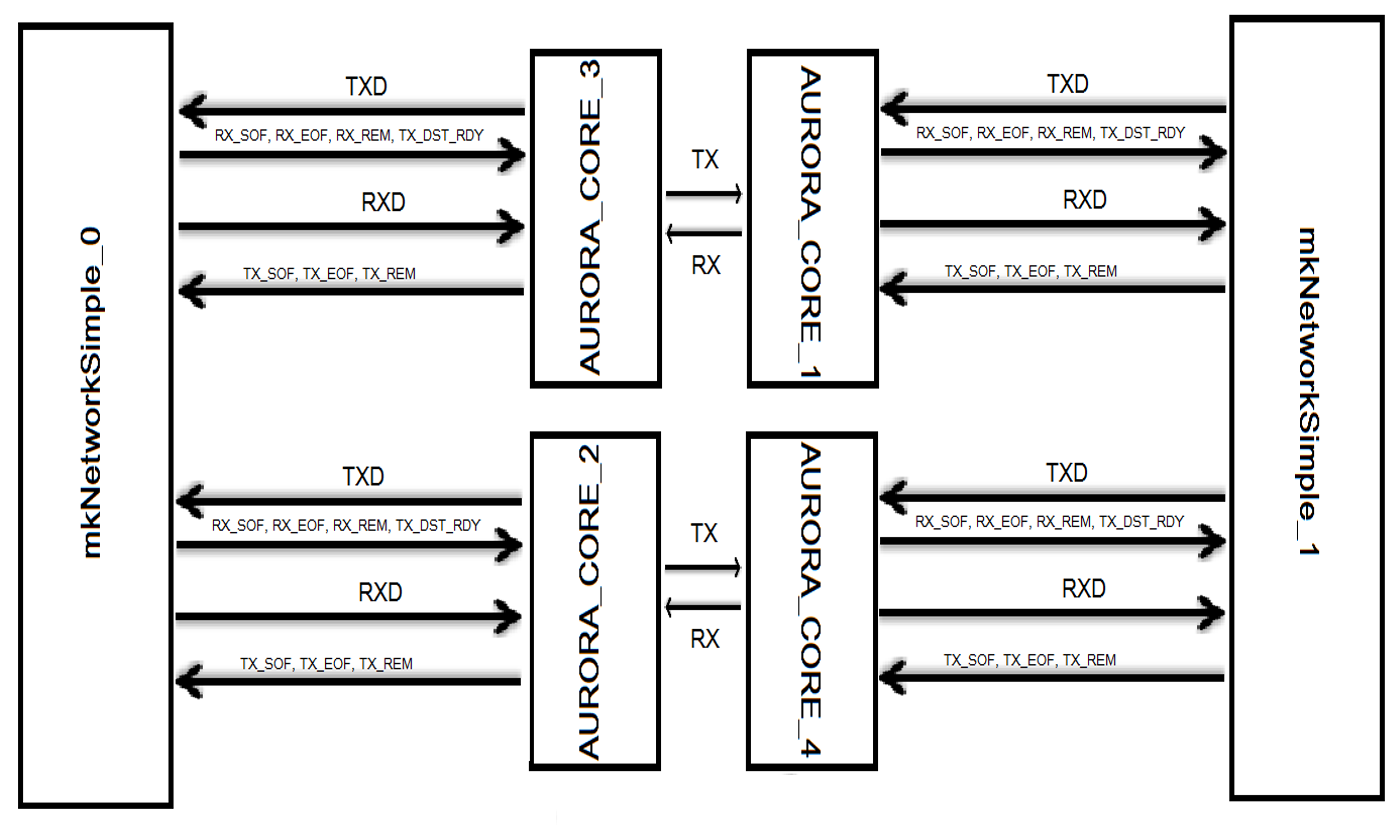
\includegraphics[scale=1]{./figs/PartitioningArchitecture}
  \caption{\textbf{Inter connected partitioned network architecture}}
  \label{PartitioningArchitecture}
\end{figure}
\end{centering}

\section{NoC partitioning using automated methods}

\begin{itemize} 
	\item{Routers: List containing all router id’s in the NoC to be partitioned.}
	\item{Part: List containing the router id’s in the partition.}
	\item{Part\_no: Partition number.}
	\item{Ports\_per\_router: Number of ports in the router module.}
	\item{Flit\_data\_width: Flit data width in the CONNECT generated NoC (can also be looked up in \textit{connect\_paramters.v}).}
	\item{vc\_bits: Number of bits for virtual channels (Should be 1 for non-VC networks. Can be looked up in \textit{connect\_paramters.v}).}
	\item{dest\_bits: Bits required for specifying port address (logarithm of number of end/receive ports in the Network).}
	\item{hex\_filename: Prefix of the .hex files generated for routing tables by the CONNECT tool.}
\end{itemize}
Usage: Place the input NoC file mkNetworkSimple.v in the same directory.\\
\textit{
Command: python mkNetworkScript.py\\
Output: Output partitioned network file mkNetworkSimple\_(part\_no).v\\
}
\begin{lstlisting}
########## Python script Parameters for automatic partitioning #############
import re
routers = [0, 1, 2, 3]		# Total No. of router in partitioned network
part = [0, 1, 2] 				# No. of router in this partitioned network
part_no = 0 					# Partition part No.
ports_per_router = 3 		# No. of ports in each router of partitioned network
flit_data_width = 16 		# Data width
vc_bits = 1
dest_bits = 2					# destination width depending on no. of ports
data_width = 2
hex_filename = <Routing_table_<filename. Hex>
######### This script partition's the given network and instantiate ########
########### all the necessary Quasi-SERDES link interfaces using wire ##########
####################### to appropriate counterpart #########################
\end{lstlisting}

\section{Mesh 2 $\times$ 2 NoC Partitioning with Quasi-SERDES Link module Instantiation}

Consider a CONNECT generated 2 $\times$ 2 mesh NoC with 5 ports per router, flit width 16. A simple input queue type router with flow control type as peek flow control. 

The generated NoC top level module \textit{``mkNetworkSimple.v"} is provided as a input to the python script. By running the script with parameter setting given above in the python code segment creates mkNetworkSimple\_0.v and mkNetworkSimple\_1.v. In the Figure \ref{PartitionedNoC2x2Mesh} shows the partitioned 2 $\times$ 2 mesh NoC with Quasi-SERDES interface instantiated which is generated after automated partitioning. 

\begin{centering}
\begin{figure}[H]
  \centering
   \includegraphics[scale=0.7]{./figs/PartitionedNoC2x2Mesh}
  \caption{\textbf{Partitioned Mesh 2 $\times$ 2 NoC}}
  \label{PartitionedNoC2x2Mesh}
\end{figure}
\end{centering}

\subsection{Application Node}
The utilization of NoC for implementation of any application isolates the application from the communication protocol needed for the data exchange within the application and also from the external nodes.

Let us consider a simple application where each node is an adder that adds the received data with the input data and moves it forward to the next router in a round robin fashion. In this partitioned NoC the modules are synchronized externally by a hard reset. 

\subsection{Test Cases}
We here will try to verify the working of the partitioned NoC for a number of test case that will give us the performance of operation and clearly indicate the difference between partitioned and un-partitioned NoC implementation.
\subsubsection{Case I:} Each part of the NoC is running at same clock speeds that are perfectly synchronized. This is an most suitable scenario for an un-partitioned NoC but a difficult one for partitioned NoC due to the synchronization issue between two independent clock sources.
\begin{figure}[H]
  \centering
   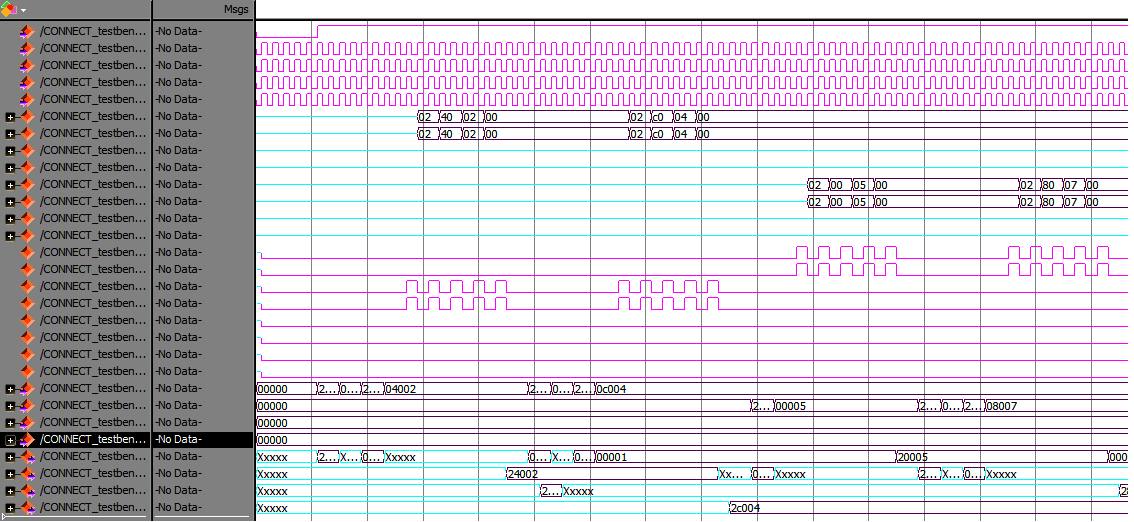
\includegraphics[scale=0.5]{./figs/SameClockTest}
  \caption{\textbf{Simulation Result for perfectly synchronous clock}}
  \label{SameCloclTest}
\end{figure}

\subsubsection{Case II:} Each part of the NoC is running at different clock speeds that are not synchronized. This is a mostly likely scenario for partitioned NoC.
\begin{figure}[H]
  \centering
   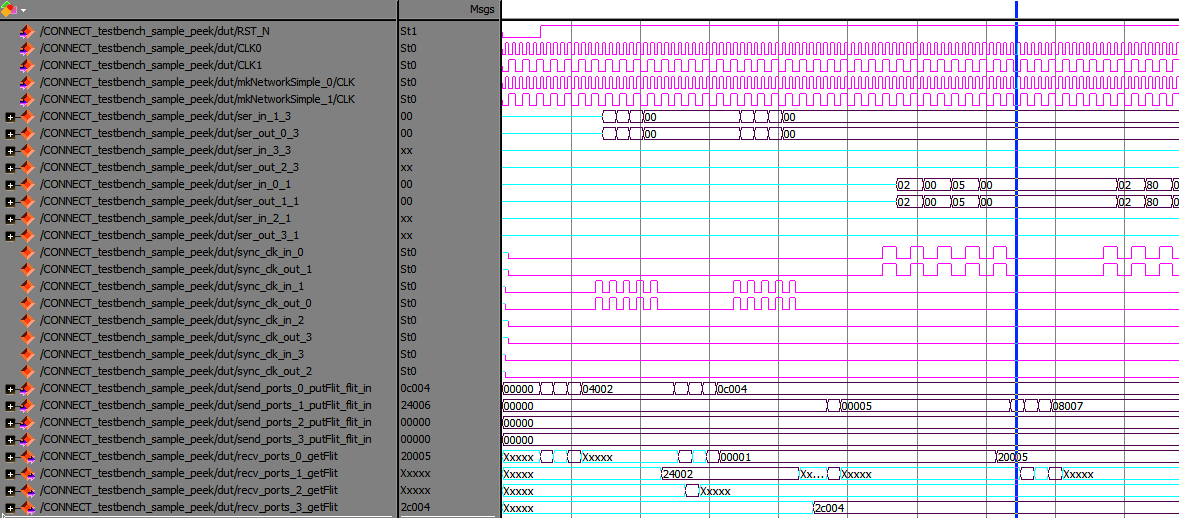
\includegraphics[scale=0.5]{./figs/DifferentClockTest}
  \caption{\textbf{Simulation Result for asynchronous clock}}
  \label{DifferentClockTest}
\end{figure}

\subsubsection{Case III:} Each part of the NoC is running at different clock speeds and are 180\textsuperscript{o} out of phase. This scenario is similar to the earlier case where the clock sources are inverted.  
\begin{figure}[H]
  \centering
   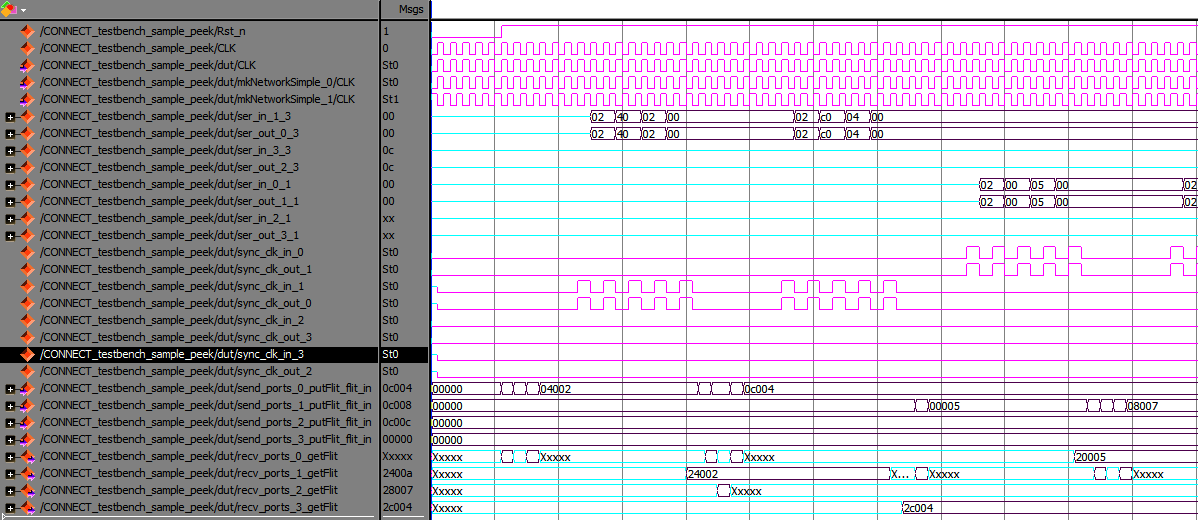
\includegraphics[scale=0.5]{./figs/OutofPhaseTest}
  \caption{\textbf{Simulation Result for 180\textsuperscript{o} out of phase Clock}}
  \label{OutofPhaseTest}
\end{figure}

To simulate and implement the above test we used a Quasi-SERDES link interface module which is discussed in chapter 5. The above simulation provides convincing results and ensures GALS type architecture will work and if it doesn't work mismatch in the clock should be a unlikely reason for the failure during implementation. A few reasons could be, the wire connecting the two boards might be interfering with each other, connections betweens boards might be getting loose as there are many wires.